\documentclass[tikz,border=7pt]{standalone}
% Shared pastel academic grammar for final-size technical-paper diagrams.
\usepackage[T1]{fontenc}
\usepackage{lmodern}
\usepackage{amsmath,amssymb}
\usepackage{xcolor}
\usepackage{tikz}
\usetikzlibrary{
  arrows.meta,
  backgrounds,
  calc,
  circuits.logic.US,
  decorations.pathreplacing,
  fit,
  matrix,
  patterns,
  positioning,
  shapes.geometric,
  shapes.symbols
}

\definecolor{ink}{RGB}{24,24,28}
\definecolor{midink}{RGB}{96,96,104}
\definecolor{paleink}{RGB}{184,184,190}
\definecolor{wash}{RGB}{241,240,237}
\definecolor{paper}{RGB}{255,255,253}
\definecolor{cyan}{RGB}{126,203,218}
\definecolor{cyanwash}{RGB}{211,238,242}
\definecolor{pink}{RGB}{235,139,158}
\definecolor{pinkwash}{RGB}{250,211,217}
\definecolor{purple}{RGB}{166,50,150}
\definecolor{purplewash}{RGB}{232,196,227}
\definecolor{gold}{RGB}{177,139,45}
\definecolor{goldwash}{RGB}{239,226,183}
\definecolor{slate}{RGB}{116,133,145}
\definecolor{slatewash}{RGB}{221,226,229}
\colorlet{muted}{midink}
\colorlet{rule}{paleink}
\colorlet{accent}{purple}
\colorlet{accentwash}{purplewash}
\colorlet{second}{cyan}
\colorlet{secondwash}{cyanwash}

\tikzset{
  every picture/.style={
    font=\rmfamily\footnotesize,
    text=ink,
    line cap=round,
    line join=round,
    >=Stealth
  },
  every node/.style={outer sep=0pt},
  panel mark/.style={font=\rmfamily\bfseries\footnotesize},
  primary/.style={font=\rmfamily\footnotesize},
  secondary/.style={font=\rmfamily\scriptsize,text=midink},
  signal name/.style={font=\ttfamily\footnotesize,anchor=east},
  scope trace/.style={draw=ink,line width=.62pt,line cap=butt,line join=miter},
  hairline/.style={draw=paleink,line width=.28pt,line cap=butt},
  dotted guide/.style={draw=midink,line width=.32pt,densely dotted},
  dashed scope/.style={draw=ink,line width=.45pt,dashed},
  transition/.style={-{Stealth[length=1.8mm,width=1.25mm]},draw=ink,line width=.58pt},
  transition label/.style={font=\rmfamily\scriptsize,fill=paper,inner sep=1.2pt},
  preedge/.style={circle,draw=ink,fill=paper,line width=.58pt,minimum size=8.2mm,inner sep=1pt},
  observed preedge/.style={preedge,fill=purplewash,double,double distance=1.15pt,line width=.62pt,minimum size=9.8mm},
  brace/.style={decorate,decoration={brace,mirror,amplitude=3pt},draw=ink,line width=.45pt},
  grid rule/.style={draw=slate,line width=.32pt,line cap=butt},
  outer rule/.style={draw=ink,line width=.82pt,line cap=butt,line join=miter},
  star mark/.style={star,star points=5,star point ratio=2.2,draw=ink,fill=purple,minimum size=5.1mm,inner sep=0pt},
  % Compatibility vocabulary used by the repository's other figures.
  flow/.style={-{Latex[length=4.5pt,width=3.2pt]},draw=ink,line width=.55pt},
  heavy flow/.style={-{Latex[length=5pt,width=3.6pt]},draw=ink,line width=.8pt},
  wire/.style={draw=ink,line width=.5pt},
  bus/.style={draw=ink,line width=1.05pt},
  guide/.style={draw=midink,line width=.4pt,dotted},
  alternate/.style={draw=ink,line width=.5pt,dashed},
  scope/.style={draw=ink,line width=.5pt,dashed,inner sep=6pt},
  block/.style={draw=ink,line width=.55pt,fill=paper,minimum height=8mm,inner xsep=5pt,inner ysep=4pt,align=center},
  operation/.style={block,fill=cyanwash,minimum width=17mm},
  register/.style={block,fill=paper,minimum width=16mm,minimum height=10mm},
  state/.style={circle,draw=ink,line width=.55pt,fill=cyanwash,minimum size=8mm,inner sep=1pt,align=center},
  terminal/.style={state,fill=purplewash,double,double distance=1.2pt,line width=.6pt},
  predicate/.style={diamond,aspect=1.8,draw=ink,line width=.55pt,fill=pinkwash,inner xsep=3pt,inner ysep=2pt,align=center},
  datum/.style={rectangle,draw=ink,line width=.5pt,fill=goldwash,minimum width=8mm,minimum height=6mm,inner sep=2pt,align=center},
  panel label/.style={font=\rmfamily\bfseries\footnotesize},
  local heading/.style={font=\rmfamily\bfseries\footnotesize},
  annotation/.style={font=\rmfamily\scriptsize,text=midink,align=center},
  heading/.style={font=\rmfamily\bfseries\small},
  subheading/.style={font=\rmfamily\bfseries\footnotesize},
  note/.style={font=\rmfamily\scriptsize,text=midink},
  label/.style={font=\rmfamily\bfseries\scriptsize},
  mono/.style={font=\ttfamily\footnotesize},
  tiny mono/.style={font=\ttfamily\scriptsize},
  count/.style={font=\rmfamily\bfseries\small},
  selected/.style={draw=ink,fill=purplewash,line width=.8pt},
  cell on/.style={fill=purple,draw=ink,line width=.3pt},
  cell off/.style={fill=paper,draw=paleink,line width=.3pt}
}

% Flat pastel facets and depth edges for restrained axonometric constructions.
\tikzset{
  cyan facet/.style={draw=ink,fill=cyanwash,line width=.5pt,line join=round},
  cyan side/.style={draw=ink,fill=cyan,line width=.5pt,line join=round},
  pink facet/.style={draw=ink,fill=pinkwash,line width=.5pt,line join=round},
  pink side/.style={draw=ink,fill=pink,line width=.5pt,line join=round},
  purple facet/.style={draw=ink,fill=purplewash,line width=.55pt,line join=round},
  purple side/.style={draw=ink,fill=purple,line width=.55pt,line join=round},
  gold facet/.style={draw=ink,fill=goldwash,line width=.5pt,line join=round},
  gold side/.style={draw=ink,fill=gold,line width=.5pt,line join=round},
  context facet/.style={draw=ink,fill=slatewash,line width=.45pt,line join=round},
  depth edge/.style={draw=midink,line width=.38pt},
  surface grid/.style={draw=slate,line width=.32pt},
  projection/.style={draw=midink,line width=.38pt,densely dashed},
  accent curve/.style={draw=purple,line width=1.05pt},
  cyan curve/.style={draw=cyan!70!ink,line width=.9pt},
  pink curve/.style={draw=pink!70!ink,line width=.9pt},
  gold curve/.style={draw=gold!80!ink,line width=.9pt}
}


\tikzset{
  probe source/.style={datum,minimum width=29mm,minimum height=7.5mm},
  support result/.style={
    register,
    fill=purplewash,
    minimum width=60mm,
    minimum height=13mm
  },
  map caption/.style={font=\rmfamily\footnotesize,text=ink,align=center},
  figure note/.style={font=\rmfamily\scriptsize,text=ink,align=center},
  legend text/.style={font=\rmfamily\scriptsize,text=ink,anchor=west},
  manifold count/.style={font=\rmfamily\bfseries\footnotesize,text=ink,align=center},
  phase label/.style={font=\rmfamily\scriptsize,text=ink,align=center},
  region letter/.style={font=\rmfamily\bfseries\scriptsize,text=ink,inner sep=.5pt},
  assumption box/.style={
    draw=ink,
    fill=paper,
    dashed,
    line width=.48pt,
    rounded corners=1pt,
    text width=51mm,
    align=left,
    inner xsep=7pt,
    inner ysep=6pt
  },
  literal branch/.style={
    -{Stealth[length=2mm,width=1.35mm]},
    draw=gold!82!ink,
    line width=.82pt
  },
  selected branch/.style={
    -{Stealth[length=2mm,width=1.35mm]},
    draw=purple,
    line width=1.02pt
  }
}

\colorlet{supporttone}{purple}

\newcommand{\supportprint}[2]{%
  % Two offset leaves provide depth while the readable mask stays orthographic.
  \path[fill=slate!18,draw=midink,line width=.28pt]
    (.15,-.15) rectangle ({11*#1+.15},{-11*#1-.15});
  \path[fill=supporttone!18!paper,draw=ink,line width=.34pt]
    (.075,-.075) rectangle ({11*#1+.075},{-11*#1-.075});
  \path[fill=paper] (0,0) rectangle ({11*#1},{-11*#1});
  \foreach \i in {#2} {
    \pgfmathtruncatemacro{\gr}{int(\i/11)}
    \pgfmathtruncatemacro{\gc}{mod(\i,11)}
    \path[fill=supporttone!68!ink]
      ({\gc*#1},{-\gr*#1}) rectangle ++(#1,-#1);
  }
  \foreach \k in {0,...,11} {
    \draw[draw=slate,line width=.28pt]
      (0,{-#1*\k}) -- ({11*#1},{-#1*\k});
    \draw[draw=slate,line width=.28pt]
      ({#1*\k},0) -- ({#1*\k},{-11*#1});
  }
  \draw[draw=ink,line width=.62pt] (0,0) rectangle ({11*#1},{-11*#1});
}

\newcommand{\paintcells}[3]{%
  \foreach \i in {#2} {
    \pgfmathtruncatemacro{\gr}{int(\i/11)}
    \pgfmathtruncatemacro{\gc}{mod(\i,11)}
    \path[fill=#3] ({\gc*.30},{-\gr*.30}) rectangle ++(.30,-.30);
  }
}

\newcommand{\mapgrid}{%
  \foreach \k in {0,...,11} {
    \draw[draw=slate,line width=.28pt]
      (0,{-.30*\k}) -- (3.30,{-.30*\k});
    \draw[draw=slate,line width=.28pt]
      ({.30*\k},0) -- ({.30*\k},-3.30);
  }
  \draw[draw=ink,line width=.68pt] (0,0) rectangle (3.30,-3.30);
}

\begin{document}
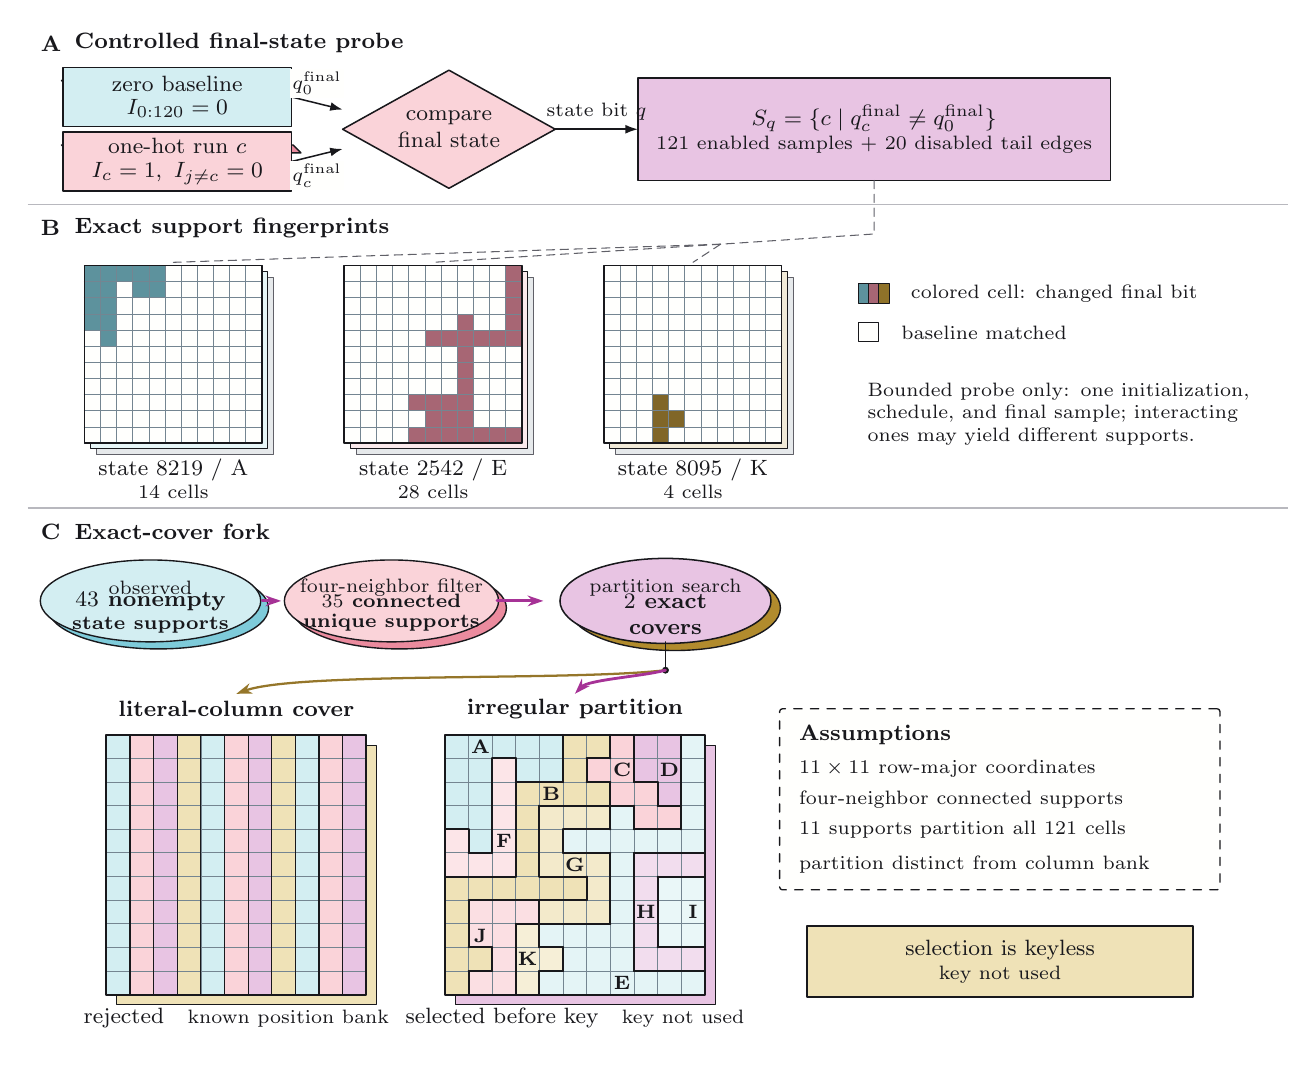
\begin{tikzpicture}[x=1cm,y=1cm]
  \path[use as bounding box] (0,.20) rectangle (16,-12.78);

  % A. Controlled runs are two leaves projected onto one final-state section.
  \node[panel label,anchor=west] at (.05,0) {A};
  \node[local heading,anchor=west] at (.48,0) {Controlled final-state probe};

  \path[cyan side]
    (.43,-.47) -- (3.37,-.47) -- (3.47,-.57) -- (.53,-.57) -- cycle;
  \node[probe source,fill=cyanwash] (zero) at (1.90,-.68)
    {zero baseline\\[-1pt]$I_{0:120}=0$};
  \path[pink side]
    (.43,-1.29) -- (3.37,-1.29) -- (3.47,-1.39) -- (.53,-1.39) -- cycle;
  \node[probe source,fill=pinkwash] (hot) at (1.90,-1.50)
    {one-hot run $c$\\[-1pt]$I_c=1,\ I_{j\ne c}=0$};

  \node[predicate,minimum width=27mm,minimum height=15mm] (compare) at (5.35,-1.09)
    {compare\\final state};
  \node[support result] (support) at (10.75,-1.09)
    {$\displaystyle S_q=\{c\mid q_c^{\rm final}\ne q_0^{\rm final}\}$\\[-1pt]
     \scriptsize $121$ enabled samples $+\ 20$ disabled tail edges};

  \draw[flow] (zero.east) --
    node[figure note,fill=paper,inner sep=1pt,above=2pt] {$q_0^{\rm final}$}
    ($(compare.west)+(0,.25)$);
  \draw[flow] (hot.east) --
    node[figure note,fill=paper,inner sep=1pt,below=2pt] {$q_c^{\rm final}$}
    ($(compare.west)+(0,-.25)$);
  \draw[flow] (compare.east) -- node[figure note,above] {state bit $q$} (support.west);

  \draw[hairline,line width=.42pt] (0,-2.05) -- (16,-2.05);

  % B. The three exact masks are orthographic faces of offset support sheets.
  \node[panel label,anchor=west] at (.05,-2.34) {B};
  \node[local heading,anchor=west] at (.48,-2.34) {Exact support fingerprints};

  \coordinate (projection hub) at (8.80,-2.55);
  \draw[projection] (support.south) -- (10.75,-2.42) -- (projection hub);
  \draw[projection] (projection hub) -- (1.85,-2.78);
  \draw[projection] (projection hub) -- (5.15,-2.78);
  \draw[projection] (projection hub) -- (8.45,-2.78);

  \begin{scope}[shift={(.72,-2.82)}]
    \colorlet{supporttone}{cyan}
    \supportprint{.205}{0,1,2,3,4,11,12,14,15,22,23,33,34,45}
  \end{scope}
  \node[map caption] at (1.85,-5.53)
    {state 8219 / A\\[-1pt]\scriptsize 14 cells};

  \begin{scope}[shift={(4.02,-2.82)}]
    \colorlet{supporttone}{pink}
    \supportprint{.205}{10,21,32,40,43,49,50,51,52,53,54,62,73,84,92,93,94,95,104,105,106,114,115,116,117,118,119,120}
  \end{scope}
  \node[map caption] at (5.15,-5.53)
    {state 2542 / E\\[-1pt]\scriptsize 28 cells};

  \begin{scope}[shift={(7.32,-2.82)}]
    \colorlet{supporttone}{gold}
    \supportprint{.205}{91,102,103,113}
  \end{scope}
  \node[map caption] at (8.45,-5.53)
    {state 8095 / K\\[-1pt]\scriptsize 4 cells};

  \path[fill=cyan!68!ink,draw=ink,line width=.3pt]
    (10.55,-3.05) rectangle (10.68,-3.30);
  \path[fill=pink!68!ink,draw=ink,line width=.3pt]
    (10.68,-3.05) rectangle (10.81,-3.30);
  \path[fill=gold!78!ink,draw=ink,line width=.3pt]
    (10.81,-3.05) rectangle (10.94,-3.30);
  \node[legend text] at (11.10,-3.18) {colored cell: changed final bit};
  \path[fill=paper,draw=ink,line width=.3pt]
    (10.55,-3.54) rectangle (10.80,-3.79);
  \node[legend text] at (10.98,-3.67) {baseline matched};
  \node[figure note,anchor=north west,text width=50mm,align=left]
    at (10.55,-4.20)
    {Bounded probe only: one initialization, schedule, and final sample; interacting ones may yield different supports.};

  \draw[hairline,line width=.42pt] (0,-5.90) -- (16,-5.90);

  % C. The connected supports are a subset; partition search then yields two covers.
  \node[panel label,anchor=west] at (.05,-6.20) {C};
  \node[local heading,anchor=west] at (.48,-6.20) {Exact-cover fork};

  \path[cyan side] (1.66,-7.17) ellipse (1.40 and .52);
  \path[cyan facet] (1.56,-7.08) ellipse (1.40 and .52);
  \node[phase label] at (1.56,-6.91) {observed};
  \node[manifold count] at (1.56,-7.23)
    {$43$ nonempty\\[-1pt]\scriptsize state supports};

  \path[pink side] (4.72,-7.17) ellipse (1.36 and .52);
  \path[pink facet] (4.62,-7.08) ellipse (1.36 and .52);
  \node[phase label,font=\rmfamily\scriptsize] at (4.62,-6.91)
    {four-neighbor filter};
  \node[font=\rmfamily\bfseries\scriptsize,align=center] at (4.62,-7.23)
    {$35$ connected\\[-1pt]unique supports};

  \path[gold side] (8.22,-7.17) ellipse (1.34 and .54);
  \path[purple facet] (8.10,-7.08) ellipse (1.34 and .54);
  \node[phase label] at (8.10,-6.91) {partition search};
  \node[manifold count] at (8.10,-7.25) {$2$ exact\\covers};
  \draw[selected branch] (2.98,-7.08) -- (3.22,-7.08);
  \draw[selected branch] (5.96,-7.08) -- (6.55,-7.08);

  \coordinate (cover fork) at (8.10,-7.96);
  \draw[wire] (8.10,-7.60) -- (cover fork);
  \fill[ink] (cover fork) circle (1.25pt);
  \draw[literal branch] (cover fork)
    .. controls (6.90,-8.10) and (3.42,-7.98) .. (2.65,-8.26);
  \draw[selected branch] (cover fork)
    .. controls (7.80,-8.04) and (7.12,-8.08) .. (6.95,-8.26);

  \node[local heading] at (2.65,-8.45) {literal-column cover};
  \begin{scope}[shift={(1.00,-8.78)}]
    \path[fill=goldwash,draw=ink,line width=.35pt]
      (.13,-.13) rectangle (3.43,-3.43);
    \path[fill=paper] (0,0) rectangle (3.30,-3.30);
    \foreach \c in {0,4,8} {
      \path[fill=cyanwash] ({.30*\c},0) rectangle ++(.30,-3.30);
    }
    \foreach \c in {1,5,9} {
      \path[fill=pinkwash] ({.30*\c},0) rectangle ++(.30,-3.30);
    }
    \foreach \c in {2,6,10} {
      \path[fill=purplewash] ({.30*\c},0) rectangle ++(.30,-3.30);
    }
    \foreach \c in {3,7} {
      \path[fill=goldwash] ({.30*\c},0) rectangle ++(.30,-3.30);
    }
    \mapgrid
    \foreach \c in {1,...,10} {
      \draw[draw=ink,line width=.42pt] ({.30*\c},0) -- ({.30*\c},-3.30);
    }
  \end{scope}
  \node[map caption] at (2.65,-12.38)
    {rejected\quad\scriptsize known position bank};

  \node[local heading] at (6.95,-8.45) {irregular partition};
  \begin{scope}[shift={(5.30,-8.78)}]
    \path[fill=purplewash,draw=ink,line width=.35pt]
      (.13,-.13) rectangle (3.43,-3.43);
    \path[fill=paper] (0,0) rectangle (3.30,-3.30);
    \paintcells{A}{0,1,2,3,4,11,12,14,15,22,23,33,34,45}{cyanwash}
    \paintcells{B}{5,6,16,25,26,27,28,36,47,58,66,67,68,69,70,71,77,88,99,100,110}{goldwash}
    \paintcells{C}{7,17,18,29,30,41,42}{pinkwash}
    \paintcells{D}{8,9,19,20,31}{purplewash}
    \paintcells{E}{10,21,32,40,43,49,50,51,52,53,54,62,73,84,92,93,94,95,104,105,106,114,115,116,117,118,119,120}{cyanwash!62!paper}
    \paintcells{F}{13,24,35,44,46,55,56,57}{pinkwash!58!paper}
    \paintcells{G}{37,38,39,48,59,60,61,72,81,82,83}{goldwash!72!paper}
    \paintcells{H}{63,64,65,74,85,96,107,108,109}{purplewash!58!paper}
    \paintcells{I}{75,76,86,87,97,98}{cyanwash!48!paper}
    \paintcells{J}{78,79,80,89,90,101,111,112}{pinkwash!72!paper}
    \paintcells{K}{91,102,103,113}{goldwash!55!paper}
    \mapgrid
    \foreach \xa/\ya/\xb/\yb in {
      1/4/1/5,1/7/1/9,1/10/1/11,2/1/2/5,2/9/2/10,
      3/1/3/6,3/8/3/11,4/3/4/6,4/7/4/9,4/10/4/11,
      5/0/5/2,5/4/5/5,5/9/5/10,6/1/6/2,6/6/6/7,
      7/0/7/1,7/2/7/4,7/5/7/8,8/0/8/2,8/3/8/4,
      8/5/8/10,9/2/9/3,9/6/9/9,10/0/10/4,
      2/1/3/1,6/1/7/1,3/2/5/2,6/2/7/2,8/2/9/2,
      4/3/8/3,9/3/10/3,0/4/1/4,5/4/7/4,8/4/10/4,
      1/5/2/5,5/5/7/5,8/5/11/5,0/6/3/6,4/6/6/6,
      9/6/11/6,1/7/6/7,3/8/7/8,1/9/2/9,4/9/5/9,
      9/9/11/9,1/10/2/10,4/10/5/10,8/10/11/10
    } {
      \draw[draw=ink,line width=.72pt]
        ({.30*\xa},{-.30*\ya}) -- ({.30*\xb},{-.30*\yb});
    }
    \foreach \x/\y/\letter in {
      1.5/.5/A,4.5/2.5/B,7.5/1.5/C,9.5/1.5/D,7.5/10.5/E,
      2.5/4.5/F,5.5/5.5/G,8.5/7.5/H,10.5/7.5/I,
      1.5/8.5/J,3.5/9.5/K
    } {
      \node[region letter] at ({.30*\x},{-.30*\y}) {\letter};
    }
  \end{scope}
  \node[map caption] at (6.95,-12.38)
    {selected before key\quad\scriptsize key not used};

  \node[assumption box,anchor=north west] at (9.55,-8.45)
    {\textbf{Assumptions}\\[4pt]
     \scriptsize $11\times11$ row-major coordinates\\[3pt]
     \scriptsize four-neighbor connected supports\\[3pt]
     \scriptsize $11$ supports partition all $121$ cells\\[3pt]
     \scriptsize partition distinct from column bank};
  \node[block,fill=goldwash,minimum width=49mm,minimum height=9mm]
    at (12.35,-11.66)
    {selection is keyless\\[-1pt]\scriptsize key not used};
\end{tikzpicture}
\end{document}
